%-----------------------------------LICENSE------------------------------------%
%   This file is part of tikz_figures.                                         %
%                                                                              %
%   tikz_figures is free software: you can redistribute it and/or              %
%   modify it it under the terms of the GNU General Public License as          %
%   published by the Free Software Foundation, either version 3 of the         %
%   License, or (at your option) any later version.                            %
%                                                                              %
%   tikz_figures is distributed in the hope that it will be useful,            %
%   but WITHOUT ANY WARRANTY; without even the implied warranty of             %
%   MERCHANTABILITY or FITNESS FOR A PARTICULAR PURPOSE.  See the              %
%   GNU General Public License for more details.                               %
%                                                                              %
%   You should have received a copy of the GNU General Public License along    %
%   with tikz_figures.  If not, see <https://www.gnu.org/licenses/>.           %
%------------------------------------------------------------------------------%

% Use the standalone class for displaying the tikz image on a small PDF.
\documentclass[crop, tikz]{standalone}

% Import the tikz package to use for the drawing.
\usepackage{tikz}

% Needed for blackboard bold C.
\usepackage{amssymb}

% The arrow package is used for the LaTeX arrow.
\usetikzlibrary{arrows.meta}

% Used for a shorter minus symbol.
\DeclareMathSymbol{\minus}{\mathbin}{AMSa}{"39}

% Begin the document.
\begin{document}

    % Draw the picture.
    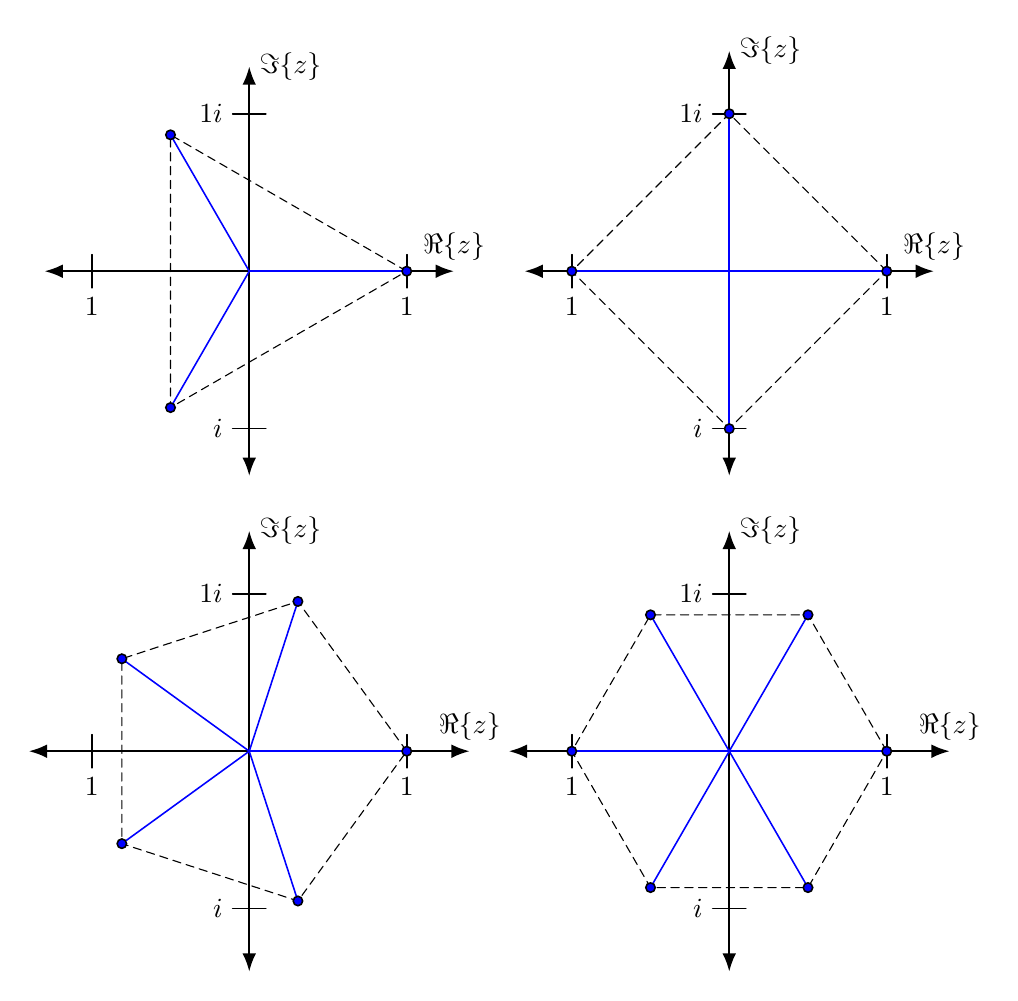
\begin{tikzpicture}[%
        > = Latex,
        line width = 0.2mm,
        line cap = round,
        scale = 2.0
    ]

        % Draw the cubed roots of unity.
        \begin{scope}[xshift = -0.6in]

            % Coordinates for the three roots and origin.
            \coordinate (O)  at (0.0, 0.0);
            \coordinate (Z1) at (1.0, 0.0);
            \coordinate (Z2) at (-0.5, 0.866);
            \coordinate (Z3) at (-0.5, -0.866);

            % Axes:
            \begin{scope}[thick]
                \draw[<->] (-1.3, 0) to (1.3, 0) node[above] {$\Re\{z\}$};
                \draw[<->] (0, -1.3) to (0, 1.3) node[right] {$\Im\{z\}$};
            \end{scope}

            % Axes labels:
            \draw (1, 3pt)  to (1, -3pt)  node [below] {$1$};
            \draw (-1, 3pt) to (-1, -3pt) node [below] {$\minus{1}$};
            \draw (3pt, 1)  to (-3pt, 1)  node [left]  {$1{i}$};
            \draw (3pt, -1) to (-3pt, -1) node [left]  {$\minus{i}$};

            % Draw the cubed roots of unity.
            \draw[blue] (O) to (Z1);
            \draw[blue] (O) to (Z2);
            \draw[blue] (O) to (Z3);

            % Connect the three roots with dashed lines.
            \draw[densely dashed, thin] (Z1) to (Z2) to (Z3) to cycle;

            % Draw dots to mark the points.
            \draw[fill = blue] (Z1) circle (0.3mm);
            \draw[fill = blue] (Z2) circle (0.3mm);
            \draw[fill = blue] (Z3) circle (0.3mm);
        \end{scope}

        % Draw the fourth roots of unity.
        \begin{scope}[xshift = 0.6in]

            % Coordinates for the four roots.
            \coordinate (O)  at ( 0.0,  0.0);
            \coordinate (Z1) at ( 1.0,  0.0);
            \coordinate (Z2) at ( 0.0,  1.0);
            \coordinate (Z3) at (-1.0,  0.0);
            \coordinate (Z4) at ( 0.0, -1.0);

            % Axes.
            \begin{scope}[thick]
                \draw[<->] (-1.3, 0) to (1.3, 0) node [above] {$\Re\{z\}$};
                \draw[<->] (0, -1.3) to (0, 1.4) node [right] {$\Im\{z\}$};
            \end{scope}

            % Axes labels.
            \draw (1, 3pt)  to (1, -3pt)  node [below] {$1$};
            \draw (-1, 3pt) to (-1, -3pt) node [below] {$\minus{1}$};
            \draw (3pt, 1)  to (-3pt, 1)  node [left]  {$1{i}$};
            \draw (3pt, -1) to (-3pt, -1) node [left]  {$\minus{i}$};

            % Draw the quartic roots of unity.
            \draw[blue] (O) to (Z1);
            \draw[blue] (O) to (Z2);
            \draw[blue] (O) to (Z3);
            \draw[blue] (O) to (Z4);

            % Draw dashed lines connecting the roots.
            \draw[densely dashed, thin] (Z1) to (Z2) to (Z3) to (Z4) to cycle;

            % Draw dots to mark the points.
            \draw[fill = blue] (Z1) circle (0.3mm);
            \draw[fill = blue] (Z2) circle (0.3mm);
            \draw[fill = blue] (Z3) circle (0.3mm);
            \draw[fill = blue] (Z4) circle (0.3mm);
        \end{scope}

        % Draw the fifth roots of unity.
        \begin{scope}[xshift = -0.6in, yshift = -1.2in]

            % Coordinates for the five roots.
            \coordinate (O)  at (0, 0);
            \coordinate (Z1) at (1, 0);
            \coordinate (Z2) at (0.309, 0.951);
            \coordinate (Z3) at (-0.809, 0.587);
            \coordinate (Z4) at (-0.809, -0.587);
            \coordinate (Z5) at (0.309, -0.951);

            % Axes.
            \begin{scope}[thick]
                \draw[<->] (-1.4, 0) to (1.4, 0) node[above] {$\Re\{z\}$};
                \draw[<->] (0, -1.4) to (0, 1.4) node[right] {$\Im\{z\}$};
            \end{scope}

            % Axes labels.
            \draw (1, 3pt)  to (1, -3pt)  node [below] {$1$};
            \draw (-1, 3pt) to (-1, -3pt) node [below] {$\minus{1}$};
            \draw (3pt, 1)  to (-3pt, 1)  node [left]  {$1{i}$};
            \draw (3pt, -1) to (-3pt, -1) node [left]  {$\minus{i}$};

            % Draw the fifth roots of unity.
            \draw[blue] (O) to (Z1);
            \draw[blue] (O) to (Z2);
            \draw[blue] (O) to (Z3);
            \draw[blue] (O) to (Z4);
            \draw[blue] (O) to (Z5);

            % Draw dashed lines connecting the roots.
            \draw[densely dashed, thin]
                (Z1) to (Z2) to (Z3) to (Z4) to (Z5) to cycle;

            % Draw circles to mark the five roots.
            \draw[fill = blue] (Z1) circle (0.3mm);
            \draw[fill = blue] (Z2) circle (0.3mm);
            \draw[fill = blue] (Z3) circle (0.3mm);
            \draw[fill = blue] (Z4) circle (0.3mm);
            \draw[fill = blue] (Z5) circle (0.3mm);
        \end{scope}

        % Draw the sixth roots of unity.
        \begin{scope}[xshift = 0.6in, yshift = -1.2in]

            % Coordinates for the six roots.
            \coordinate (O)  at (0, 0);
            \coordinate (Z1) at (1, 0);
            \coordinate (Z2) at (0.5, 0.866);
            \coordinate (Z3) at (-0.5, 0.866);
            \coordinate (Z4) at (-1, 0);
            \coordinate (Z5) at (-0.5, -0.866);
            \coordinate (Z6) at (0.5, -0.866);

            % Axes:
            \begin{scope}[thick]
                \draw[<->] (-1.4, 0) to (1.4, 0) node [above] {$\Re\{z\}$};
                \draw[<->] (0, -1.4) to (0, 1.4) node [right] {$\Im\{z\}$};
            \end{scope}

            % Axes labels:
            \draw (1, 3pt) to (1, -3pt)   node [below] {$1$};
            \draw (-1, 3pt) to (-1, -3pt) node [below] {$\minus{1}$};
            \draw (3pt, 1)  to (-3pt, 1)  node [left]  {$1{i}$};
            \draw (3pt, -1) to (-3pt, -1) node [left]  {$\minus{i}$};

            % Draw the sixth roots of unity.
            \draw[blue] (O) to (Z1);
            \draw[blue] (O) to (Z2);
            \draw[blue] (O) to (Z3);
            \draw[blue] (O) to (Z4);
            \draw[blue] (O) to (Z5);
            \draw[blue] (O) to (Z6);

            % Draw dashed lines connecting the roots.
            \draw[densely dashed, thin]
                (Z1) to (Z2) to (Z3) to (Z4) to (Z5) to (Z6) to cycle;

            % Draw dots marking the roots.
            \draw[fill = blue] (Z1) circle (0.3mm);
            \draw[fill = blue] (Z2) circle (0.3mm);
            \draw[fill = blue] (Z3) circle (0.3mm);
            \draw[fill = blue] (Z4) circle (0.3mm);
            \draw[fill = blue] (Z5) circle (0.3mm);
            \draw[fill = blue] (Z6) circle (0.3mm);
        \end{scope}
    \end{tikzpicture}
\end{document}
